\documentclass[twoside,10pt]{article}
\usepackage{/Users/bradenhoagland/latex/styles/toggles}
%\toggletrue{sectionbreaks}
%\toggletrue{sectionheaders}
\newcommand{\docTitle}{Math 412 - HW 5}
\usepackage{/Users/bradenhoagland/latex/styles/common}
\importStyles{modern}{rainbow}{boxy}

%\renewcommand{\theenumi}{\alph{enumi}}

\begin{document}
%\tableofcontents

% ------------------------------
% Lesson 9, 10 points
% ------------------------------
\begin{exer}[Lesson 9, 10 points]
Denote by $K$ the simplicial complex on page $7$ of Lesson $9$ and $f$ the given filtration. Find a simplicial complex $L$ and filtration $h$ such that $(K, f)$ and $(L, h)$ have the same degree-$1$ Betti number at every time but different dimension $1$ persistence modules. In symbols, prove there exists a filtered complex $(L, h)$ such that $\beta_1(K^t) = \beta_1(L^t)$ for every $t \in \R$ but $H_1(f) \neq H_1(g)$.

	Do the analogous exercise as above for $p=2$. That is, find two filtered simplicial complexes $(K, f)$ and $(L, h)$ and prove $\beta_2(K^t) = \beta_2(L^t)$ for every $t \in \R$ but $H_2(f) \neq H_2(g)$.
\end{exer}

\textbf{First part:} In class we proved that the given complex had first homology $H_1(f) = I_{[4,7)} \oplus I_{[5,\infty)}$. Now consider the following filtration on the same complex: the black integers are the original filtration $h$, and the colored integers are the modified filtration to be used with the algorithm for computing simplicial homology.

\begin{figure}[H]
	\centering
	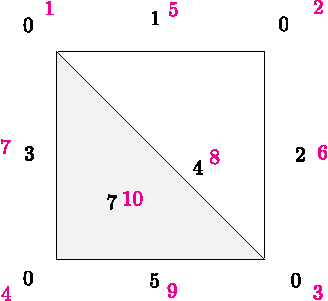
\includegraphics[scale=1]{fig/1a.pdf}
	%\caption{}
\end{figure}

The persistent homology algorithm starts with the following matrix (I don't include columns for the vertices since those will only affect the 0th homology, not the 1st; missing values are implicitly 0).
\begin{center}
	\begin{tabular}{c|c c c c c c}
		& 5&6&7&8&9&10 \\
		\hline
		1& 1&0&1&1&0&0\\
		2& 1&1&0&0&0&0\\
		3& &1&0&1&1&0\\
		4& &&1&&1&0\\
		5& &&&&&0\\
		6& &&&&&0\\
		7& &&&&&1\\
		8& &&&&&1\\
		9& &&&&&1\\
		10& &&&&&0
	\end{tabular}
\end{center}
After applying the algorithm, this reduces to the following.
\begin{center}
        \begin{tabular}{c|c c c c c c}
                & 5&6&7&8&9&10 \\
                \hline
                1& 1&0&1&&&0\\
                2& 1&1&0&&&0\\
                3& &1&0&&&0\\
                4& &&1&&&0\\
                5& &&&&&0\\
                6& &&&&&0\\
                7& &&&&&1\\
                8& &&&&&1\\
                9& &&&&&1\\
                10& &&&&&0
        \end{tabular}
\end{center}
Thus the 1st homology for the modified filtration is $I_{[9,10)}\oplus I_{[8,\infty)}$, which for the original filtration $h$ corresponds to
\[
	H_1(h) = I_{[5,7)}\oplus I_{[4,\infty)}.
\] Note that this is different than $H_{1}(f)$, yet $\beta_1(K^{t}) = \beta_1(L^{t})$ for all $t$ since both 1st homologies have the same dimension at every time $t$.


\textbf{Second half:} We'll use a similar strategy for the 2nd homology. Take two tetrahedrons (one with a void inside and one filled in) and identity a face of one to a face of the other. In the figure below, all faces (although not drawn) are present, the pink edges represent the solid tetrahedron, and the blue edges represent the hollow tetrahedron.

\begin{figure}[H]
	\centering
	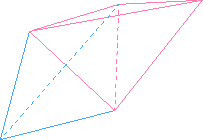
\includegraphics[scale=1.5]{fig/1b.pdf}
	%\caption{}
\end{figure}

We can put two different filtrations on it: $f$ sends all vertices to $-1$, all blue edges and faces to $0$, all pink edges and faces to $1$, and the solid bit inside the pink tetrahedron to $2$. The filtration $g$ sends the vertices and solid pink bit to the same values, but now sends all blue edges and faces to $1$ and all pink edges and faces to $0$.

For $g$, we can modify the filtration to work with the persistent homology algorithm as follows (I've split up the complex below to make it easier to tell what's being labeled with what; I also don't bother to relabel the vertices, as they won't affect the algorithm for the 2nd homology).

\begin{figure}[H]
	\centering
	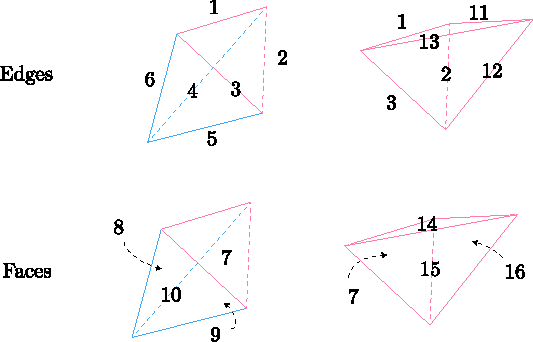
\includegraphics[scale=1.4]{fig/1c.pdf}
	%\caption{}
\end{figure}

Not pictured above is the solid bit inside the pink tetrahedron, which is mapped to 17. This gives us a massive matrix to use in the algorithm. I don't include columns for the vertices or edges, as these won't affect $H_2$.
\begin{center}
	\begin{tabular}{c|c c c c c c c c}
		& 7&8&9&10&14&15&16&17 \\
		\hline
		1& 1&1&0&0&1&0&0&0 \\
		2& 1&0&1&0&0&0&1&0 \\
		3& 1&0&0&1&0&1&0&0 \\
		4&  &1&1&0&0&0&0&0 \\
		5&  &0&1&1&0&0&0&0 \\
		6&  &1& &1&0&0&0&0 \\
		7&  & & & &0&0&0&1 \\
		11& & & & &1&0&1&0 \\
		12& & & & &0&1&1&0 \\
		13& & & & &1&1& &0 \\
		14& & & & & & & &1 \\
		15& & & & & & & &1 \\
		16& & & & & & & &1
	\end{tabular}
\end{center}
The algorithm turns this into the following.
\begin{center}
        \begin{tabular}{c|c c c c c c c c}
                & 7&8&9&10&14&15&16&17 \\
                \hline
                1& 1&1&0& &1&1& &0 \\
                2& 1&0&1& &0&0& &0 \\
                3& 1&0&0& &0&1& &0 \\
                4&  &1&1& &0&0& &0 \\
                5&  &0&1& &0&0& &0 \\
                6&  &1& & &0&0& &0 \\
                7&  & & & &0&0& &1 \\
                11& & & & &1&1& &0 \\
                12& & & & &0&1& &0 \\
                13& & & & &1& & &0 \\
                14& & & & & & & &1 \\
                15& & & & & & & &1 \\
                16& & & & & & & &1
        \end{tabular}
\end{center}
Thus the 2nd homology for the modified filtration is $I_{[16,17)}\oplus I_{[10,\infty)}$, which corresponds to
\[
	H_2(f) = I_{[1,2)}\oplus I_{[0,\infty)}.
\] Repeating this process for the filtration $g$, we get
\[
	H_2(g) = I_{[0,2)}\oplus I_{[1,\infty)}
\] instead. Once again, these are different persistence diagrams, yet their dimension is the same at all times.

\newpage

% ------------------------------
% Lesson 9, 5 points
% ------------------------------
\begin{exer}[Lesson 9, 5 points]
Let $\{[b_i, d_i)\}_{i=1}^m$ be an arbitrary collection of half-open intervals. Prove there exist a simplicial complex $K$ with filtration $f$ such that $H_1(f) = \oplus_{i=1}^m I_{[b_i, d_i)}$. Hint: Consider the algorithm for computing persistent homology. 
\end{exer}

Consider the following filtered (with filtration $f$) simplicial complex, where all vertices are mapped by $f$ to $\min_i\left\{ b_i \right\}- 1$.
\begin{figure}[H]
	\centering
	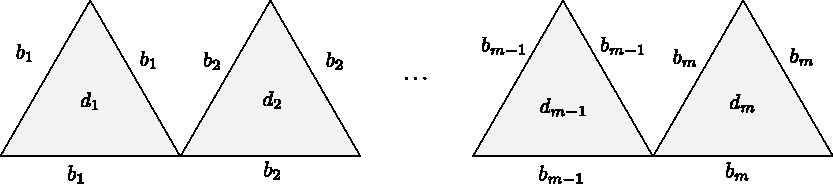
\includegraphics[scale=0.9]{fig/2a.pdf}
	%\caption{}
\end{figure}

We claim that this filtered complex has first homology group $H_1(f)\cong \bigoplus_{i=1}^{m}I_{[b_i,d_i)} $. First note that since $m$ is finite, we can assume without loss of generality that $\left\{ b_i \right\}$ is nondecreasing in $i$. This allows us to introduce a new filtration $g$, whose values on each vertex are shown below.

\begin{figure}[H]
	\centering
	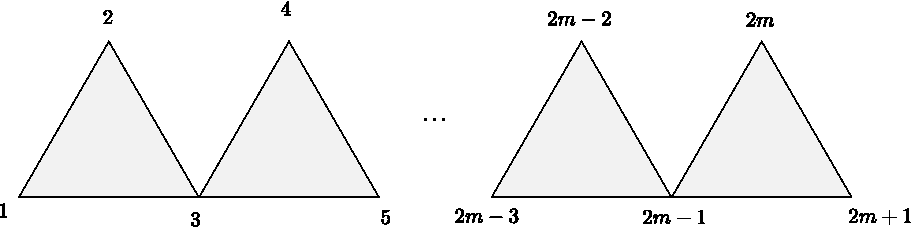
\includegraphics[scale=0.9]{fig/2b.pdf}
	%\caption{}
\end{figure}

Note that we cannot determine where $g$ maps the edges of all but the first triangle, nor can we determine where it maps the faces of any triangle. Instead, we'll use the following convention on where $g$ maps the edges and face of the $i$-th triangle.

\begin{figure}[H]
	\centering
	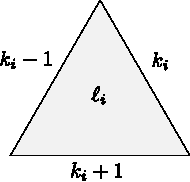
\includegraphics[scale=1]{fig/2c.pdf}
	%\caption{}
\end{figure}

This new filtration $g$ is compatible with our algorithm for computing persistent homology, so we can use it to determine the intervals that make up $H_1(g)$, then use this to deduce $H_1(f)$. The $i$-th triangle contributes the following columns to the matrix $M$ in the algorithm, where any empty spaces or missing rows/columns are zero.
\begin{center}
	\begin{tabular}{c|c c c c c}
		& $k_i-1$ & $k_i$ & $k_i+1$ & $\cdots$ & $\ell_i$ \\
		\hline
		$2i-1$ & 1 & 0 & 1 \\
		$2i$ & 1 & 1 & 0 \\
		$2i+1$ & 0 & 1 & 1 \\
		$\vdots$ \\
		$k_i-1$ & & & & & 1 \\
		$k_i$ & & & & & 1 \\
		$k_i+1$ & & & & & 1
	\end{tabular}
\end{center}

This particular subset of $M$ reduces to the following.
\begin{center}
        \begin{tabular}{c|c c c c c}
                & $k_i-1$ & $k_i$ & $k_i+1$ & $\cdots$ & $\ell_i$ \\
                \hline
                $2i-1$ & 1 & 0 & {\color{blue}0} \\
                $2i$ & 1 & 1 & {\color{blue}0} \\
                $2i+1$ & 0 & 1 & {\color{blue}0} \\
                $\vdots$ \\
                $k_i-1$ & & & & & 1 \\
                $k_i$ & & & & & 1 \\
                $k_i+1$ & & & & & 1
        \end{tabular}
\end{center}

Since $g$ is injective and no two faces in our complex share the same edge, the \textit{only} row with $\text{low}(i,M) = k_i+1$ is $i=\ell_i$. Similarly, the only columns with $\text{low}(i,M) = 2i+1$ are $i=k_i$ and $i=k_i+1$. Thus the four columns introduced by the $i$-th triangle only interact with each other during the algorithm. This means that the only intervals composing $H_1(g)$ are $I_{[k_i+1,\ell_i)}$, which correspond in $H_1(f)$ to $I_{[b_i,d_i)}$. Thus our complex has the desired first homology group.

\newpage

\end{document}
